\documentclass{book}
\usepackage{graphicx}
\usepackage{url}
\usepackage{csquotes}
\usepackage{textcomp}
\usepackage{menukeys}
\usepackage[hang,flushmargin]{footmisc} 
\graphicspath{ {images/} }
% listings package and parameters provide formatting for
% source code examples
\usepackage{listings}
\usepackage{color}
\definecolor{dkgreen}{rgb}{0,0.6,0}
\definecolor{gray}{rgb}{0.5,0.5,0.5}
\definecolor{mauve}{rgb}{0.58,0,0.82}
\lstset{frame=tb,
	language=Python,
	aboveskip=3mm,
	belowskip=3mm,
	showstringspaces=false,
	columns=flexible,
	basicstyle={\small\ttfamily},
	numbers=left,
	numberstyle=\tiny\color{black},
	keywordstyle=\color{black},
	commentstyle=\color{dkgreen},
	stringstyle=\color{black},
	breaklines=true,
	breakatwhitespace=true,
	tabsize=3
}
\begin{document}
\frontmatter
\pagestyle{plain}
\begin{titlepage}
	\title {\huge \textbf{Introduction to Accounting Data Analytics Using Python}}
	\date{First Edition}
	\author{Stephen Perreault, PhD, CPA}
	\maketitle
\end{titlepage}
% copyright page
\begingroup
	\parindent 0pt
	\parskip \baselineskip 
	\textcopyright{} 2017 Stephen J. Perreault 
	
	\begin {center}
	
\includegraphics  [scale=1.5]{creative_commons_license}
	\end {center}
	
	This work is licensed under the Creative Commons Attribution-NonCommercial-NoDerivatives 4.0 International License. To view a copy of this license, visit http://creativecommons.org/licenses/by-nc-nd/4.0/ or send a letter to Creative Commons, PO Box 1866, Mountain View, CA 94042, USA.
	
	First edition: August 2017
\endgroup
\tableofcontents

% acknowlegments
\begin {center}
\newpage
\textit{
To Kathleen, Lyla, Willy, and Matilda.}
\end {center}

\mainmatter	
\parindent 0pt
\parskip \baselineskip 

% Chapter 1
\chapter{Introduction}
\section{What is data analytics?}
\section{Sources of data}
\section{About this book}
\section{Intended audience}
\section{Software used}
Assumes you are using a Windows-based PC. Mac versions in the future.

% Chapter 2

\chapter{Version control}
\section{Why you should care about version control}

Imagine that the audit engagement team which you have been assigned to is in need of a tool that can assess the valuation of an audit client's stock options using the Black-Scholes-Merton valuation model.\footnote{It's not important to understand what the Black-Scholes-Merton model is to appreciate this example. However, if you're curious, BSM can be used, among other things, to determine the price of certain types of stock options.} The tool needs to be simple to use, scalable, and compatible with a wide variety of operating systems. Knowing your reputation as a skilled programmer who works well under pressure, your supervisor has given you 24 hours to write the Python script to perform this assessment.

You spend the night hunched over your keyboard working frantically to complete the assigned task before the deadline. Your source code undergoes numerous changes as you squash bugs, improve performance, and add extra features that you believe the engagement team might find useful. As the sun begins to rise the next morning, you realize that you have successfully completed the task. You have developed a functional software tool that you are sure will impress your supervisor. 

Before emailing the Python script to the engagement team, you decide to make some minor tweaks to your code in order to slightly improve the tool's performance. After making the seemingly harmless modification to your code, you test the script one final time and are horrified to discover that the change you made has caused an error which has rendered the program non-functional.

Frantically, you scan through the script, hoping to identify the changes that you made which might have caused the program to break. You haphazardly remove a few lines of code that you think may be the culprit but that doesn't seem to do the trick - the program still crashes. In addition, this deletion causes another portion of the program to break. Feeling hopelessly lost, you begin to realize that you may be forced to start the project from scratch. What will you possibly tell your supervisor?

As the example above has hopefully demonstrated, it is incredibly important for programmers to keep track of the changes made to their source code over time. This process can seem daunting, especially for large projects with many different developers working on the code base simultaneously. Fortunately, modern developers can rely on version control systems to help manage these changes. If an error is introduced into the code, the developer can simply turn back the clock and revert to an earlier stable version. 

Since we're going to be writing a significant amount of computer code as we work our way through this book, it makes sense to start by learning a bit about how version control works. In this chapter we will learn how to use version control to track changes to our individual projects. We will also learn how to create an online repository of our source code which can be shared with others and used as an online software development portfolio.

\section{Introducing Git}

In this book we will be using the widely used and popular version control system Git\texttrademark. Git was created in 2005 by Linus Torvalds, the famous creator of the popular operating system Linux. In addition to providing developers with a history of all the individual changes that have been made to their projects, Git can also be used to track changes for developers working collaboratively. 

As an example, let's say that you and a coworker have been assigned the task of writing a piece of software and will both need access to the source code during development. To facilitate this, you could post the code on a shared network drive or a file hosting service that you and your coworker can access. This method would probably work just fine unless the two of you are working on the same code file at the same time. If that happens, one of you would have your work overwritten and erased. Git can keep that from happening. If you and your coworker are both making changes to the same source code file, Git will save two copies. Later on, the changes can be merged together without losing any of the earlier work. 

Unfortunately, Git has an reputation as being difficult for beginners to use (which is undeserved in my humble opinion). This mostly stems from the fact that it does not have a graphical user interface; rather, users access the features of Git by typing in commands using the system terminal or command line. While there are GUI tools available for Git, working from the command line is an important skill set for an aspiring Python programmer to develop. As a result, we will be using the command line when working with Git in this book. 

\section{Introducing GitHub}

While Git is handy version control system for working with projects locally on our computers, there are often times when we want to share our projects with others. To do this, we'll be using the online service GitHub\texttrademark. GitHub is basically an online social media service; however, the primary type of information being shared on GitHub is source code as opposed to cat pictures!\footnote{This attempt at humor is actually not factually correct - projects posted on GitHub can contain images if the user wishes.} Throughout this book, we'll be using GitHub and Git in tandem in order to manage changes and share our projects with others.

\begin{figure}[h]
	\caption{Registering for a GitHub account}
	\centering\includegraphics[width=.90\textwidth]{/Chapter2/Figure_1}
\end{figure}

Although desktop clients are available, GitHub can be used without installing any software onto our computers. You simply have to sign up for a free GitHub account. Let's go ahead and do that now by visiting \texttt{https://github.com}. The sign up process is as easy as registering for any other social network. Note that you'll want to sign up for the free plan. GitHub also offers paid subscriptions with more advanced features; however, these features our unnecessary for the purposes of this book.

I encourage you to personalize your GitHub profile by uploading a recent picture of yourself. You may also wish to include  other relevant background information  or links to a webpage (if you have one). However, remember that the information which you include in your profile is publicly viewable - only provide information you would be comfortable sharing with others, including future employers. Once you're finished, let's move on to installing Git.

\section{Installing Git}

If you are using a computer that is connected to a campus network (such as a machine in an on-campus computer lab), there is a good chance that Git is already installed.\footnote{If you see an entry for ``Git Bash" somewhere on the computer's Windows Start Menu, then Git is already installed.} However, if you plan on working through this book using your personal computer (which is probably the case) you will need to install Git on that device.

You can find the installation package on Git's homepage which is located at \texttt{https://git-scm.com/downloads}. Download the Windows release and then open the executable. Accept all default installation settings by clicking "Next" until the installer begins extracting the program files to your hard drive. Once the installation is complete, you should be able to find a folder called ``Git" within the Windows start menu. Inside the folder you should see a shortcut to a program called ``Git Bash." Clicking this shortcut will launch the Git command line. Let's go ahead and do that now.

\begin{figure}[h]
	\caption{The Git homepage showing the link to the installation package}
	\centering\includegraphics[width=1\textwidth]{/Chapter2/Figure_2}
\end{figure}

Launching ``Git Bash'' for the first time will display an empty terminal window which should look a bit like Figure 2.2. The first line of output in the terminal should contain your Windows account name as well the hostname of the computer you are using (we will be ignoring this information). The dollar sign (\$) represents the terminal prompt which is where we will be typing all of our Git commands.

\begin{figure}[h]
	\caption{An empty Git Bash terminal}
	\centering\includegraphics[width=.90\textwidth]{/Chapter2/Figure_3}
\end{figure}

With the terminal open, let's go ahead and tell Git who we are. Type in the following command:\\ \\ \texttt{git config -- global user.name "My Name"}

Obviously, you'll need to replace the words in quotation marks with your own name! You can use your full name, a nickname, or a handle that you regularly use online. Git will attribute any changes you make to projects to the name that you provide here. You'll also need to provide Git with your email address (make sure it's the same email address you used when signing up for GitHub) using the following command: \\ \\ \texttt{git config --global user.email "my\_email@my\_email.com"}

\section{Creating your first repository}

Both GitHub and Git store individual projects in ``repositories" (often referred to as ``repos" for short). Any files that make up your projects (e.g., source code, image files, text files, etc.) can be stored inside a repository. Let's go ahead and create a repository right now. 

Log into your GitHub account and click the ``Create New" button (this looks like a small + sign to the left of your profile picture at the top of the webpage). Select the option to create a new repository. Name this new repository \texttt{my\_first\_repo} and leave the ``Initialize this repository with a README" box unchecked (your screen should look similar to Figure 2.4). You can also give the repository a brief description if you like. Once finished, click the ``Create repository" button. 

\begin{figure}[h]
	\caption{Creating a new repository using GitHub}
	\centering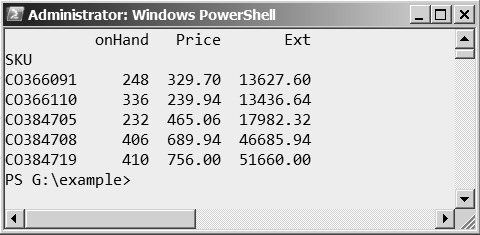
\includegraphics[width=.90\textwidth]{/Chapter2/Figure_4}
\end{figure}

You've now created a repository for your project on GitHub. However, the majority of the work you do on your projects is likely going to be performed on a local computer instead of online (for example, we want to be able to work on our projects in places where we don't have an internet connection). Therefore, we are also going to create a local repository for our project using Git. We'll link the local Git and online Github repos together later in the chapter.

Before you create a new local repository, you're going to need to create a location on your hard drive (or network drive if you're using a lab computer) where that repo will live. Re-open the Git Bash terminal and enter the command: \\ \\ \texttt{mkdir \textasciitilde/my\_first\_repository}
 
This will create a directory (or folder) called \texttt{my\_first\_repository} where your repository and its related files will be stored on the drive.\footnote{This folder will be created off of the top level directory on the drive. For most Windows users, this will be \texttt{C:\textbackslash users\textbackslash your\_user\_name}. However, it may also be the top level of the network drive if you are using a PC in a campus computer lab (e.g., \texttt{G:\textbackslash}). You can find the location of the top level directory by using the \texttt{\textasciitilde/} command.}

Now navigate to the new directory you just created using the command:

\texttt{cd my\_first\_repository}

As you may have guessed, \texttt{cd} stands for ``change directory.'' Note that if you want to navigate out of this directory and back to the top-level directory, simply use the command:

\texttt{cd}

Notice that the path displayed above the command prompt changes depending on the directory you are currently located in. This is demonstrated in Figure 2.5 (note that my top-level folder in this example is G:\textbackslash).

\begin{figure}[h]
	\caption{Navigating directories using Git Bash}
	\centering\includegraphics[width=.90\textwidth]{/Chapter2/Figure_5}
\end{figure}

Let's navigate back to the \texttt{my\_first\_repository} directory. We're now going to initialize a new Git repository in this directory by using the command:{\footnote {You can tell that this is a command which is specific to Git (as opposed to a system command such as \texttt{mkdir} or \texttt{cd}) due to the fact that is prefixed by the term \texttt{git}.}} 

\texttt{git init}

If successful, Git will tell us that it has initialized an empty repository in the filepath we have chosen. Congratulations - you have created your first Git repo!

\section{Adding files to your repository}
Now that we have created a working repository, it is time to begin adding files. Every Git repository you create should contain a file that provides a brief written overview of the project. We'll be adding a file called \texttt{README.md} to our repository which contains this information.\footnote{See \texttt{https://gist.github.com/jxson/1784669} for an excellent template for creating informative project README files.}

This \texttt{README.md} file must be created as a simple text file (which means that the file contains no data other than text). We can create such a file using any text editing tool. Since all copies of Windows come with the ``Notepad'' text editor, this is the program we will be using to create our \texttt{README.md} file. Find the Notepad program on your computer and open it (a shortcut to the program can typically be found in the Accessories folder within the Windows Start Menu).

Once Notepad has been opened, type the name of your project on the first line of the file (this is usually the same name as your repo name). Inserting the hash character (\#) prior to the project name will make this text slightly larger than the remaining text in the file. (It is good practice to prefix all section headings in your \texttt{README.md} files with \#). On a separate line of the file, provide a brief description of the project. Note that, in practice \texttt{README.md} should contain far more information than this; however, this level of description is sufficient for our current purposes. Figure 2.6 provides an example of what this file might look like.

\begin{figure}[h]
	\caption{\texttt{README.md} for the project}
	\centering\includegraphics[width=.90\textwidth]{/Chapter2/Figure_6}
\end{figure}

\begin{figure}[h]
	\caption{Saving to the repository directory}
	\centering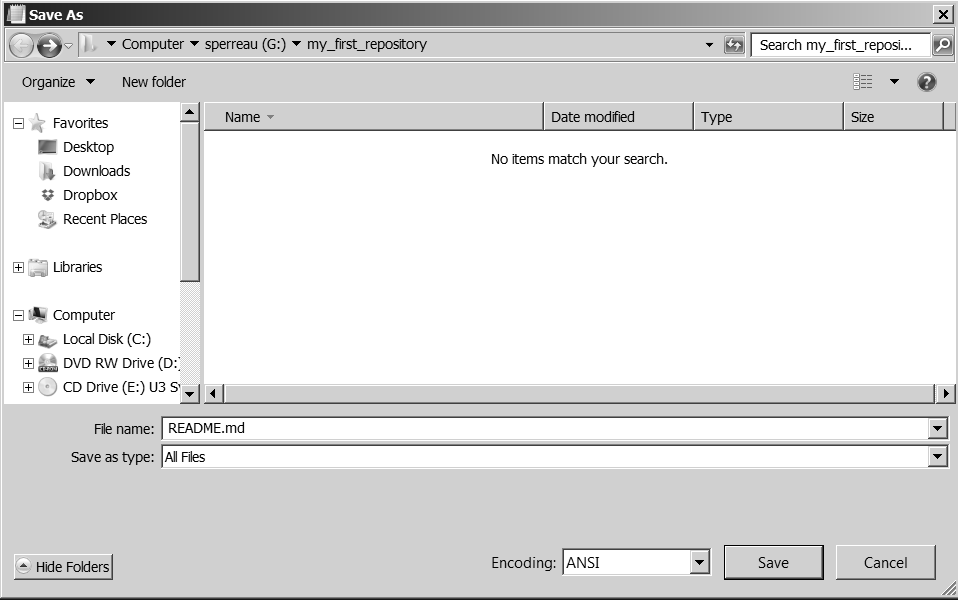
\includegraphics[width=.90\textwidth]{/Chapter2/Figure_7}
\end{figure}

When your text file looks sufficient, it's time to save it to the directory that we created our repository in. In Notepad, click ``Save as" from the ``File" dropdown menu. Then navigate to the repository directory. Type \texttt{README.md} as the ``File Name'' and click the ``Save'' button. See Figure 2.7.

We have now saved the file to the directory where we created our repository; however, we now need to specifically tell Git to add the file to our repo and begin tracking it. To do this, we'll need to re-open the Git Bash terminal. 

If necessary, navigate back to the directory where the project repository is located. Then enter the following command:

\texttt{git add README.md}

Now that the file has been added to the repository, let's check the status of the repo using the command:

\texttt{git status}

The output should look something like the output in Figure 2.8. 

\begin{figure}[h]
	\caption{Checking the repository status}
	\centering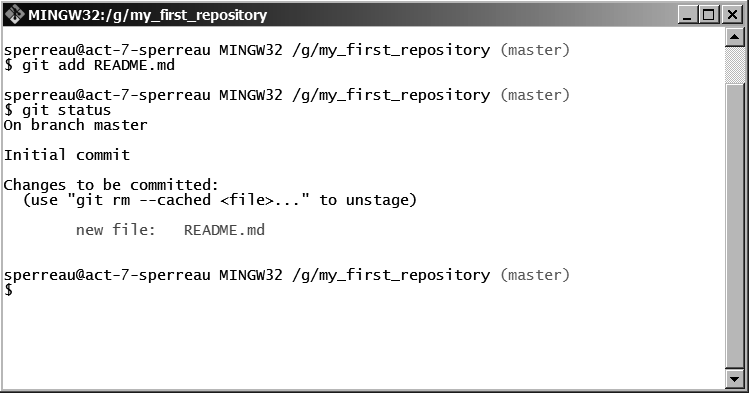
\includegraphics[width=.90\textwidth]{/Chapter2/Figure_8}
\end{figure}

Let's take some time to review this output. First, notice that Git has indicated that this repository is the ``(master)'' branch of the repository. We haven't yet created any additional branches for this project so this is to be expected. We'll talk more about incorporating multiple project branches later in the chapter.

The next line of Git output tells us that we are currently creating the ``initial" (or first)  commit for the repository. Whenever we save changes to a repository, we refer to this as ``commiting the changes" in Git parlance. Commits also provide us with a snapshot of our project at a particular point in time, allowing us to restore the project to one of these previous states if so desired. The output indicates this initial commit will involve adding a new file to the repository called \texttt{README.md}, as expected. Note that we should always check the status of our repository using \texttt{git status} prior to commiting any changes.

Since the status of our repo looks as expected, let's go ahead and commit the change. This can be done with the command:

\texttt{git commit -m "Add README.md"}

The ``commit" command tells Git to commit all pending changes to the repository. We have also included the \texttt{-m} flag to associate this commit with a brief message indicating what changes are being recorded to the repository. You should always include such messages when executing a commit so you have a record of the changes made to your project over time. You can verify that your commit worked by checking the status of the repo again using \texttt{git status}. You will notice that there are no other changes scheduled to be commited.

\section{Pushing commits to GitHub}
So far we have only modified the version of the repository that is stored locally on our individual computers. However, at some point we will likely want to share our repo online with others. We can do this by linking our Git repository to our GitHub account and ``pushing" the changes to the GitHub repository that we created earlier. Let's do this now.

We first need to tell Git that a remote (or online) version of our repository exists. We do this by providing Git with the web address (url) for our GitHub repository. The format for this address is:

\texttt{https://github.com/user\_name/repo\_name}

where \texttt{user\_name} and \texttt{project\_name} are replaced with your GitHub username and the name of your GitHub repository.

We'll point Git to this GitHub repository using the following command:

\texttt{git remote add origin https://github.com\_name/repo\_name}

The command tells Git that our project files can now be sent to a remote location (called ``origin") which can be found at the github address provided. We can verify that we have configured our repository correctly be using the following command:

\texttt{git remote -v}

The \texttt{-v} flag tells Git to provide a verbose description of the repository which contains the url name. If your repository is set up correctly, the output will look similar to Figure 2.9.

\begin{figure}[h]
	\caption{Checking the remote origins for a repository}
	\centering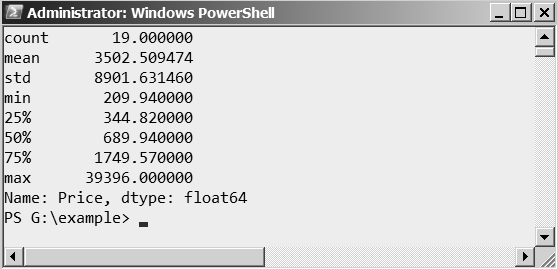
\includegraphics[width=.90\textwidth]{/Chapter2/Figure_9}
\end{figure}

Note that the origin connection is listed twice with the descriptors \texttt{(fetch)} and \texttt{(push)}. This means that we are both able to \textit{push} changes to and \textit{fetch} changes from the online GitHub repo.

Now that we've verified that our connections are configured appropriately, we can actually push our changes up to the GitHub remote. The following command tells GitHub to push the master branch of the repo (the only branch we have created so far) to the origin connection we just established. Note that you may be prompted to login to GitHub again when issuing this command.

\texttt{git push origin master}

You can verify that the push command worked successfully by visiting the GitHub repo page using your web browser. You should see that the file \texttt{README.md} has been added to the online repository and that the repo description has been appropriately updated based upon the contents of the file.

\begin{figure}[h]
	\caption{Verifying the push command on GitHub.com}
	\centering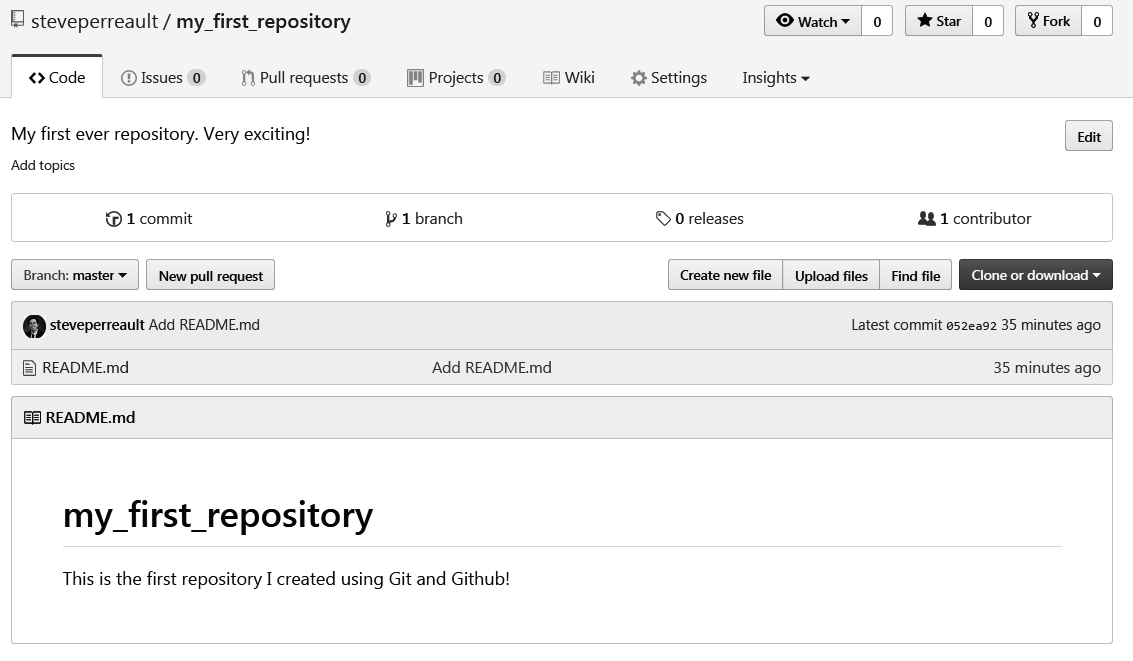
\includegraphics[width=.90\textwidth]{/Chapter2/Figure_10}
\end{figure}

\section{Reverting a commit}
Since we've only pushed one commit to the example repository we've been working with in this chapter, let's go ahead and push another one now. Open Git Bash and enter the following command from within the repository directory:

\texttt{touch badfile.bad}

\texttt{Touch} is a terminal command that creates an empty file. For this example, we simply want to make a change to the repository that we can commit. Adding a new file using the \texttt{touch} fulfills that objective nicely.

You can see the contents of the working directory by using the terminal command \texttt{ls}. Entering this command should display the following files which currently make up the repo directory: \texttt{README.md badfile.bad}.

Now, using the methods discussed in the previous two sections, perform the following steps:

\begin{itemize}
	\item Add \texttt{badfile.bad} to the local repository
	\item Check the local repository status, making sure that \texttt{badfile.bad} is marked as an addition to be commited
	\item Commit the change to the local repository with the message \texttt{"Add badfile.bad"}
	\item Push the new commit to the remote version of the repository on GitHub
\end{itemize}

Note that the GitHub remote origin connection that we established earlier is permanently associated with the repository unless we manually remove it (you can verify this with \texttt{git remote -v}). So you do not have to re-establish this connection every time you push commits for this repo to GitHub.

If you have completed these steps correctly, when you visit the repository page on GitHub.com you will see that \texttt{badfile.bad} has been added to the online repo. In addition, GitHub now tells us that two commits have been processed to this repository, as visibile in Figure 2.11.

\begin{figure}[h]
	\caption{Displaying the list of commits for a GitHub repository}
	\centering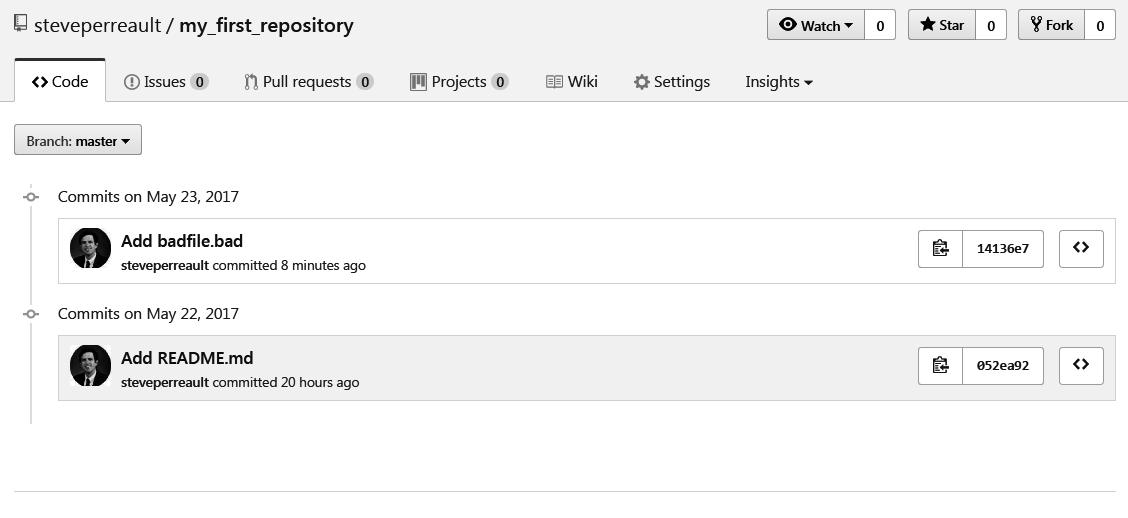
\includegraphics[width=.95\textwidth]{/Chapter2/Figure_11}
\end{figure}

There may be times when we push a commit that changes a branch in some undesirable way. For example, let's assume that the last commmit pushed to GitHub was in error and that we \textit{really} don't want \texttt{badfile.bad} to be including within the \texttt{my\_first\_repository} repo. In this instance, we may want to revert the repository back to what it looked like before we made the commit. We can do this using Git's \texttt{revert} command. We'll first revert the local repository to the earlier state using Git Bash and then we will push the modification of the local repo to GitHub.

To start, obtain a listing of all of the changes made to our local repository by using the command: \texttt{git log}.\footnote{Using the Git command \texttt{git log --oneline} will display each commit on single line. This may be useful for repositories with large numbers of commits. Also, your terminal may make your log scrollable if the output exceeds the height of its window. In this case, you can use your keyboard's arrow keys to scroll through the log. Entering \texttt{q} will return you to the terminal prompt.} For example, as seen in Figure 2.12, the log file for the  \texttt{my\_first\_repository} repo currently lists two commits (Git displays the most recent commits first). In this example, we want to revert our repo back to the state that existed immediately after the first commit where \texttt{README.md} was added. In order to maintain an accurate change history, Git treats the reversion as an additional commit.

\begin{figure}[h]
	\caption{Displaying the log file for a local repository}
	\centering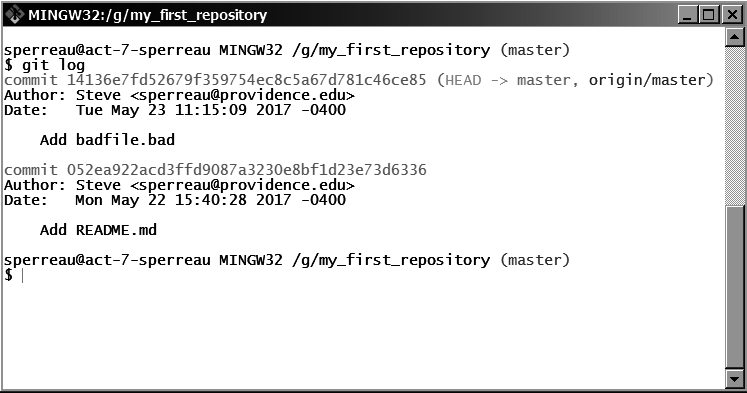
\includegraphics[width=.95\textwidth]{/Chapter2/Figure_12}
\end{figure}
 
 To do this, we'll use the following Git command:
 
 \texttt {git revert 14136e7 --no-edit}
 
 where ``14136e7" refers to the first seven digits of the identifier for commit we want to revert (Git does not require us to type the full identifier number).\footnote{Note that the identifier number you type here will be unique to your specific repository.} The \texttt{--no-edit} flag associates a default description with the reversion commit, which is sufficient for our purposes. Once the command has been entered, displaying the log file for the repository using \texttt{git log} should now show the reversion commit as the most recent entry.
 
 Now all that's left to do is to push this latest commit to GitHub using \texttt{git push origin master}. Once this has been done you will have successfully reverted the commit!

\section{Cloning a repository}
In addition to being able to ``push" a project of your own to GitHub, you can also use Git grab a copy of a repository that another GitHub user has created. This is done using Git's \texttt{clone} command.

To clone an existing repository, open Git Bash and enter the following command:

\texttt{git clone https://github/user\_name/repository\_name}

where \texttt{user\_name} and \texttt{repository\_name} represent the repository name and GitHub username associated with the repository to be cloned. Note that the \texttt{clone} command will do the following:

\begin{itemize}
	\item Create a new local folder that has the same name as the repository being cloned
	\item Initialize the new folder as a repository using \texttt{git init}
	\item Copy all of the cloned repository's files and commits to the new local folder
	\item Create a remote connection named \texttt{origin} which points to the URL where the repository was cloned from
\end{itemize}

Pay careful attention to that last bullet point. Unless you change the default remote origin connection created by \texttt{clone}, any commits you push to GitHub will be recorded to the GitHub repository that was originally cloned (the owner of the repository will need to approve the changes). 

If you want to push changes made to your locally cloned repository to \textit{your own} GitHub account (as will usually be the case), you can use the following command:

\texttt{git remote set-url origin https://github.com/user\_name/repository\_name}

where the web address reflects the URL of the GitHub repository that you want to push changes to (this will typically be an empty repository you have created in GitHub following the steps discussed earlier in the chapter).

\section{Advanced: Creating branches}
When a repository is initially created, by default it contains a single branch called the ``Master'' branch. This master branch is considered the definitive branch of the project. As such, with larger projects, changes to the master branch should be considered carefully.

However, it is possible for a repository to contain other branches which are not considered separate from the master branch. At the time of their creation, these branches contain a perfect copy of the contents of the master branch. However, because they are only a copy of the master, developers can make edits and changes to the new branch worrying about corrupting the master branch. In this way, your master branch can be insulated from inadvertent errors introduced by changes made in other branches. Ultimately, commits made in these other branches can be merged into the master branch once the changes are determined to be stable.

Let's create a new branch of the /texttt{my\_first\_repository} repository that we created earlier in the chapter. From the local directory for the repository, enter the command:

\texttt{git branch bugfix1}

where \texttt{bugfix1} represents the customizable name for the new branch.\footnote{Note that software development teams often create branches to manage specific project issues, so branch names such as \texttt{bugfix1} are somewhat common.} To switch from the master branch to the new branch you just created, use the command:

\texttt{git checkout bugfix1}

Now push this new branch to GitHub using the command we learned earlier:

\texttt{git push origin bugfix1} 

You can now verify that the separate branches have been pushed to GitHub, as demonstrated in Figure 2.13. Note that the commit history for the \texttt{bugfix1} branch also inherited any commits that were made to the master branch at the time that the \texttt{bugfix1} branch was created. However, going forward, any changes made to the master branch or the \texttt{bugfix1} branch will be tracked separately until the two branches are merged (as discussed in the next section).

\begin{figure}[h]
	\caption{Viewing branches in GitHub}
	\centering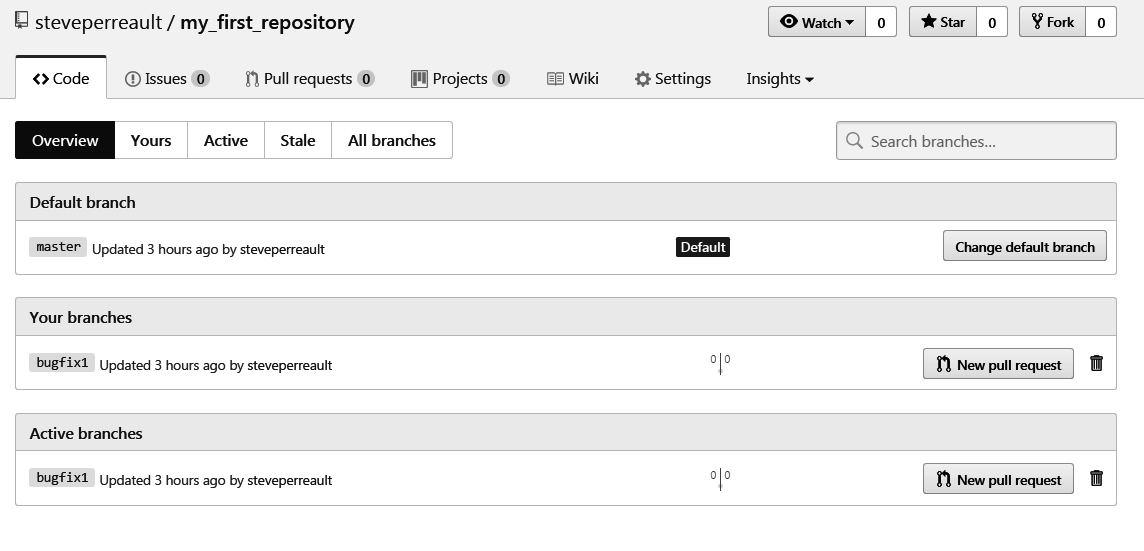
\includegraphics[width=.95\textwidth]{/Chapter2/Figure_13}
\end{figure}

We can now switch back and forth between the two branches using \texttt{git checkout} from within the terminal. We can switch between the branches in the remote repository hosted on GitHub as well. Note, however, that since our repository now contains two branches, we will need to be careful to ensure that we are working off of the \texttt{bugfix1} branch until we are ready to merge our changes into the master branch. In addition, we will need to remember to provide the appropriate branch name when pushing commits to GitHub.

It may be helpful to recall that we can use the \texttt{git status} command we discussed earlier to identify which branch is currently active within the terminal. Additionally, the command \texttt{ git branch -r} can be used to obtain a list of all remote branches for a repository.

\section{Advanced: Merging branches}

Let's see you've finished work on the \texttt{bugfix1} branch and now want to merge the changes into the master branch. To do this, switch to the branch you wish to merge into using \texttt{git checkout} (in this case, you would switch to the master branch) and enter the following command:

\texttt{git merge bugfix1}

We can then push the changes to the master branch of the remote repository on GitHub using:

\texttt{ git push origin master}]

Note that if we view the commit history for the master repository on GitHub (or locally by using \texttt{git log} within the termimal), we will that the changes made to the repository as a result of the merge are listed as a separate commit. This makes it easy to revert a merge if we so wish (we would simply follow the steps for reverting a commit discussed earlier).

For purposes of working through the exercises in this book, you should never record changes (commits) to multiple branches of a project concurrently. Doing so can cause conflicts when merging the two branches together. For example, let's say a user changes the same line of code differently within two branches that they are attempting to merge together. In this case, Git will not be able to complete the merge cleanly because it doesn't know which change is the ``correct" one to be retained. Git contains a number of features that knowledgeable users can employ in order to reconcile conflicts; however, these tools are beyond the scope of this text.

\section{Summary}
This chapter discussed the reason for using a version control system when developing your software projects. It introduced the Git package for local version control and the GitHub platform for sharing project code remotely. The concept of project repositories (repos) was introduced and the process for adding files to and making changes to repositories (commits) was discussed. The chapter described how local repositories can be stored on and retrieved from the GitHub platform. Finally, basic concepts relating to branching and merging were introduced.

Note that this chapter merely scratches the surface of what you can accomplish using Git. If you are interested in learning more about how you can use Git and GitHub in your software development projects, a good starting point would be the respective documentation for the two tools. This can be found at:

\begin{itemize}
	\item Git: \texttt{https://git-scm.com/documentation}
	\item GitHub: \texttt{https://guides.github.com}
\end{itemize}

\section{Discussion Questions}

\begin{enumerate}
	\item What is the purpose of a version control system such as Git? Mention three benefits of using such a system.
	\item Why might a developer choose to also use a social media platform such as GitHub instead of just using the Git version control system locally?
	\item Conduct some brief internet research to identify competing websites that offer services similar to GitHub. Do any such sites exist?
	\item How can the concept of branching prevent unintended problems from occurring during the software development process?
\end{enumerate}

\section{Exercises}
\begin{enumerate}
	\item Create a local repository using Git. This repository should contain:
	\begin{itemize}
		\item a README.md file which contains the name of the project and a brief description of the project. 
		\item a humorous image which you found online 
	\end{itemize}
		When finished, push the repository to your personal GitHub account.
	\item The \texttt{Ch2\_Ex2} repository located on this book's GitHub page contains a single file which includes the the text of my favorite poem. Clone a copy of this repository to your local drive and then:
	\begin{itemize}
		\item Revert the most recent commit that was made to the repo
		\item Modify the contents of \texttt{favorite\_poem.txt} so it contains the text of \textit{your} favorite poem.
	\end{itemize}
	When finished, push the modified repo to \textit {your own} GitHub account. (Note that you will need to change the URL that the origin remote connection points to in order to push to your own account!)
	\item Create a new local branch for the repository that you created in the first exercise. Then:
	\begin {itemize}
		\item Add an empty file called \texttt{addition.txt} to the new branch and commit the change.
		\item Merge the new branch into your master branch
	\end {itemize}
	When finished, push the completed project to your GitHub account.
\end{enumerate}

% Chapter 3
\chapter{Introducing Python}
\section{Why Python?}
We will be using the Python\texttrademark \ programming language to complete the data analytics tasks described in this text. The creation of Python is attributed to Guido van Rossum\footnote {Image attributed to Doc Searls (2006oscon\_203.JPG) [CC BY-SA 2.0 (http://creative commons.org/licenses/by-sa/2.0)], via Wikimedia Commons.} a Dutch programmer who wanted to create a language that was easy for beginner programmers to use but powerful enough to handle large and complex projects. Over the past several decades, Python has grown to become one of the most widely used programming languages across the globe and is regularly used by accounting data scientists and is taught in many colleges and universities. \begin{figure}[h]
	\caption{Van Rossum in 2006}
	\centering\includegraphics[width=.30\textwidth]{/Chapter3/Figure_1}
\end{figure}

Python has a number of important features which contribute to its popularity:

\begin{itemize}
	\item It's free: Python is free to use and distribute meaning that cost is not a barrier to adoption.
	\item It's open source: Python's community-based development model has resulted in the creation of thousands of third-party libraries and modules that can handle a wide variety of computing tasks. 
	\item It's easy to learn: Python has a simple structure and a clearly defined syntax. As such, it's a perfect language for beginner-level programmers.
	\item It's a "high-level" language: Python programs are abstracted from the underlying system hardware and can run on a wide variety of computers.
	\item It plays well with others: Python can easily be integrated with other programming languages such as C++ and Java.
\end{itemize}

\section{Setting up a development environment}
Our development environment will contain three specific tools:
\begin{enumerate}
	\item A text editor. We will be writing all of our source code using this editor so it is important that it can recognize Python syntax highlighting. We will be using the \textit{Notepad++} editor; however there are other options available as well. Use the editor that you are most comfortable with. 
	\item The Python interpreter. The interpreter will take the source code we write and carry out the related instructions.\footnote{We will be using the latest version of the Python 3.X interpreter which, at the time of this book's writing, is version 3.6.1. Note that the interpreter underwent a fairly controversial upgrade in 2008 which resulted in the version numbering switching from 2.7 to 3.X. The Python development team continues to support the 2.7 branch; however, it is currently scheduled to sunset in 2020 and we will not be using it in this book.}
	\item A command line shell (also referred to as a terminal). We will be using this tool to interact with the Python interpreter. The shell we will be using is Windows Powershell\textsuperscript{\textregistered}. You already have experiencing working with a command line shell from Chapter 2.
\end{enumerate}

If you are using a computer that resides on the network of a college or university campus, there is a good chance that all three of these tools are already installed on the machine you are using. However, if you will be using a personal computer, you will may need to download and install a compatible text editor and the Python interpreter (Windows PowerShell comes pre-installed on Windows version 7 and above).

\begin{itemize}
	\item The Notepad++ installer can be found at \texttt{https://notepad-plus-plus
		.org}. The installation process is straightforward and accepting all of the default installation options is sufficient.
	\item The latest version of the Python interpreter can be downloaded from 
	\texttt{https://www.python.org/downloads}. Before downloading, make sure that you don't already have Python installed on your system. To do this press \keys{Win} + \keys{R} to open the ``Run'' dialog window. In the input field, type \texttt{powershell}. Then type \texttt{python} from within the PowerShell command line window. If you see a response from the Python interpreter then Python is already installed.
	
	The Python installation process is relatively straightforward. Upon launching the installer, make sure the ``Add Python 3.X to PATH" checkbox is selected (see Figure 3.2). Then click the ``Install Now" option to proceed. The full installation will take several minutes to complete.
	
	To verify that Python has been installed, open PowerShell and type the command \texttt{python}. Python should now launch. To exit, type \texttt{quit()} and press \keys{Enter}.
\end{itemize}

\begin{figure}[h]
	\caption{The Python installer with PATH option checked}
	\centering\includegraphics[width=.90\textwidth]{/Chapter3/Figure_2}
\end{figure}

\section{Your first program: ``Hello World!"}
If you have ever learned how to code before, you have undoubtedly written a ``Hello World!" program. If not, you will embark upon this rite of new programmer passage now.

The first thing we need to do is set up a place where our new program will live. Launch PowerShell by pressing \keys{Win} + \keys{R} to open the ``Run'' dialog window. In the input field, type \texttt{powershell} to launch the terminal (you may want to create a shortcut to PowerShell so that you can access it easier in the future). We'll be using PowerShell to interact with our file system and to give commands to the Python interpreter. 

is folder will be created off of the top level directory on the drive. 

By default, PowerShell will open at the top level directory on your hard drive. If you are using a personal machine, this will likely be \texttt{C:\textbackslash users\textbackslash your\_user\_name}. However, it may also be the top level of the network drive if you are using a PC in a campus computer lab (e.g., \texttt{G:\textbackslash}). The current directory will be listed immediately prior to the \texttt{>} prompt, as shown in Figure 3.3.

\begin{figure}[h]
	\caption{The PowerShell terminal}
	\centering\includegraphics[width=.90\textwidth]{/Chapter3/Figure_3}
\end{figure}

Let's go ahead and make a directory for our first project called ``hello\_world"\footnote{I usually avoid using space characters in my directory names and filenames; however, you can use them if you wish. Note that if you elect to use space characters, you will need to encapsulate the words in quotation marks when using shell commands (e.g., \texttt{cd "hello world"}).} using the following command:

\texttt{md hello\_world}

Now change our current location to the directory we just created by typing:

\texttt{cd hello\_world}

We are now write the source code for our ``Hello World" program. In this book, we're going to always write our code in the Notepad++ text editor. Launch it now. This can be done either by selecting the application from the Windows Start Menu or it can be launched directly from within the PowerShell terminal using the command:

\texttt{start notepad++}

By default, Notepad++ should open a blank document called ``new 1" when launching for the first time. If it did not, create a new file by selecting \menu{File > New} from the menu bar. 

We now need to tell our text editor to adjust its formatting for Python syntax. We do this by selecting the following option from the menu bar: \menu{Language > P > Python}. 

Finally, let's save our blank file. From the menu bar, select \menu{File > Save as}. Navigate to the \texttt{hello\_world} directory you just created. Name the file \texttt{hello\_world}. Lastly, make sure to save the file type as ``Python file (*.py, *.pyw)."\footnote{If you correctly set the editor syntax formatting to the Python language, this file type should already be selected.} When this has been done, our new program directory should now contain an empty source code file (or script) called \texttt{hello\_world.py}. Note that the file extention \texttt{*.py} is reserved for Python scripts.

Let's now write our first lines of code. Using Notepad++, type the contents of Figure 3.4 into the \texttt{hello\_world.py} filed that you just created.

\begin{figure}[h]
	\caption{hello\_world.py}
	\begin{lstlisting}
	print ("Hello world!")
	print ("I did it! I wrote my first Python program!")
	\end{lstlisting}
\end{figure}

Note that you should not type the numbers preceding each line into your text editor. These numbers are included merely so we can reference specific lines of code later in the book. When this text has been entered correctly, save the file by pressing \keys{Ctrl} + \keys{S}. 

We have now successfully written our first Python script. We now need to test whether the Python interpreter will run it as desired. Return to PowerShell and view the contents of the \texttt{hello\_world} directory with the command \texttt{ls}. The \texttt{hello\_world.py} file that we just created should be the only contents of this directory (See Figure 3.5).\\

\begin{figure}[h]
	\caption{Contents of the \texttt{hello\_world} directory}
	\centering\includegraphics[width=.90\textwidth]{/Chapter3/Figure_5}
\end{figure}

Once you have verified that you are located in the correct directory, run the script by typing:

\texttt{python hello\_world.py}

If you have performed the steps correctly, you should see something like Figure 3.6. Congratulations! You have written your first computer program in Python!

\begin{figure}[h]
	\caption{Contents of the \texttt{hello\_world} directory}
	\centering\includegraphics[width=.90\textwidth]{/Chapter3/Figure_6}
\end{figure}

\section{A basic process for program development}

So far, we've followed a series of fairly simple steps when developing our first project. These steps are:

\begin{enumerate}
	\item Create a project folder using \texttt{mkdir}
	\item Create/modify the project's python script(s) using a text editor
	\item Test the project's script(s) using the python interpreter
\end{enumerate}

We can also easily integrate this process with the Git / GitHub version control workflow we learned about in Chapter 2. The steps involved in this integrated process are:

\begin{enumerate}
	\item Create a project folder using \texttt{mkdir}
	\item Initialize a new repository in the project folder using \texttt{git init}
	\item Create a new repository for the project on GitHub.com
	\item Link the Git repository to the remote GitHub repository using \texttt{git remote}
	\item Create the project's python script(s) using a text editor
	\item Add the scripts to the Git repository using \texttt{git add}
	\item Make the first Git commit using \texttt{git commit}
	\item Push the initial commit to GitHub using \texttt{git push}
	\item Make modifications to the Python script(s) as necessary
	\item Test project scripts using the python interpreter
	\item Commit the changes using \texttt{git commit}
	\item Push the changes to GitHub using \texttt{git push}
	\item Repeat steps 9-12 until program is complete
\end{enumerate}

Note that for simple projects, like ``Hello World", we probably wouldn't want to go through the trouble of implementing a version control system. However, as the programs we write become more complex (such as those written when completing the end of chapter exercises in this book), we probably will want to take the time to implement version control into our workflow. A side benefit of using Git / GitHub is that, as you work through the exercises in this text, you will build a shareable GitHub portfolio that demonstrates your skill in Python and accounting data analytics. 

\section{Mathematical operations}
Python supports the basic mathematical operations you are familiar with such as addition (+), subtraction (-), division (/), and multiplication (*). Within a program, they can be used like:

\begin{figure}[h]
	\caption{basic math calculations in python}
	\begin{lstlisting}
	print(3+5)
	# the answer is 8
	print(3-5)
	# the answer is -2
	\end{lstlisting}
\end{figure}

Talk about modulus, square root functions, power, etc.

\end{document}